Analiza la figura \ref{fig:lados_sem01} y encuentra la medida de $x$.

\begin{minipage}{0.45\linewidth}
    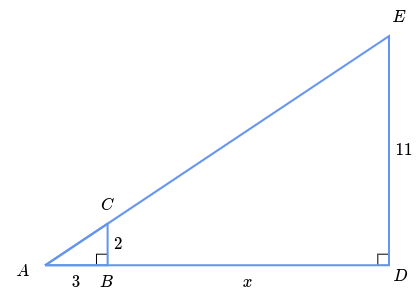
\includegraphics[width=\linewidth]{Images/lados_sem01}
    \captionof{figure}{}
    \label{fig:lados_sem01}
\end{minipage}\hfill
\begin{minipage}{0.5\linewidth}
    \begin{solutionbox}{10cm}
        Tanto $\triangle ABC$ como $\triangle ADE$ tiene un ángulo recto y comparten $\angle BAC$.\\

        $\Rightarrow$ $\triangle ABC$ y $\triangle ADE$ son semejantes.\\

        \quad $\therefore$
        \quad $\dfrac{\overline{AB}}{\overline{BC}}=\dfrac{3}{2}$ \quad y \quad $\dfrac{\overline{AD}}{\overline{DE}}=\dfrac{3+x}{11}$
        \begin{align*}
            \dfrac{3+x}{11} & =\dfrac{3}{2}  \\
            2(3+x)          & =3 (11)        \\
            6+2x            & =33            \\
            2x              & =27            \\
            x               & =\dfrac{27}{2} \\
            x               & =13.5
        \end{align*}
    \end{solutionbox}
\end{minipage}%
